% !TEX root = ../main.tex

\chapter{Theoretical Foundations}
\label{ch:theoretical}

\vspace{1cm}
\startcontents[chapters]
\minicontents
\vspace{1cm}

\emph{Part of this research has been described in a journal article in Digital Creativity in 2013, and I presented a paper at the Creativity and Cognition conference 2013 in Sydney.}

\grule % chktex 1

\begin{fcom}
  Why pataphysics? How does pataphysics relate to creativity and how does it support creativity in computers?
\end{fcom}

\begin{draft}
\begin{itemize}
  \item link the various creativity models
  \item how do they apply to computers?
  \item link pataphysics to creativity --- and computers
  \item ranking and pataphysics
  \item
\end{itemize}
\end{draft}


\section{Searching vs. Browsing}

What do we actually mean by searching? Usually it implies that there is something to be found, an \gls{in}; although that doesn’t necessarily mean that the searcher knows what he or she is looking for or how to conduct the search and satisfy that need.

From the users' point of view the search process can be broken down into four activities \autocite{Sutcliffe1998} reminiscent of classic problem solving techniques \autocite{Polya1957}:

\begin{description}
  \item [Problem identification] \gls{in},
  \item [Need articulation] \gls{in} in natural language terms,
  \item [Query formulation] translate \gls{in} into query terms, and
  \item [Results evaluation] compare against \gls{in}.
\end{description}

This model poses problems when we consider a situation where an \gls{in} cannot easily be articulated or in fact is not existent and the user is not looking for anything. This is not the only constraining factor though and Marchionini and Shneiderman have pointed out that ``the setting within which information-seeking takes place constrains the search process'' \autocite{Marchionini1988} and they laid out a framework with the following main elements.

\begin{itemize}
  \item Setting (the context of the search and external factors such as time, cost)
  \item Task domain (the body of knowledge, the subject)
  \item Search system (the database or web search engine)
  \item User (the user’s experience)
  \item Outcomes (the assessment of the results/answers)
\end{itemize}

Searching can be thought of in two ways, information lookup (\textbf{searching}) and exploratory search (\textbf{browsing}) \autocite{DeVries1993, Marchionini2006}. A situation where an \gls{in} cannot easily be articulated or in fact is not existent (the user is not looking for anything specific) can be considered a typical case of exploratory search and describes the kind of search that is most suited to our proposed tool. The former can be understood as a type of simple question answering while the latter is a more general and broad knowledge acquisition process without a clear goal.

Current web search engines are tailored for information lookup. They do really well in answering simple factoid questions relating to numbers, dates or names (e.g.\ fact retrieval, navigation, transactions, verification) but not so well in providing answers to questions that are semantically vague or require certain extend of interpretation or prediction (e.g.\ analysis, evaluation, forecasting, transformation).

When it comes to exploratory search though, the user’s success in finding the right information depends a lot more on constraining factors such as those mentioned earlier and can sometimes benefit from a combination of information lookup and exploring \autocite{Marchionini2006}.

\begin{quote}
  Much of the search time in learning search tasks is devoted to examining and comparing results and reformulat-ing queries to discover the boundaries of meaning for key concepts. Learning search tasks are best suited to combinations of browsing and analytical strategies, with lookup searches embedded to get one into the correct neighbourhood for exploratory browsing. \autocite{Marchionini2006}
\end{quote}

De Vries called this form of browsing an ``enlargement of the problem space'', where the problem space refers to the resources that possibly contain the answers/solutions to the information need \autocite{DeVries1993}. This is a somewhat similar idea to that of Boden’s conceptual spaces which she called the ``territory of structural possibilities'' and exploration of that space ``exploratory creativity'' \autocite{Boden2003}.

All of these ideas, however, seem to be concerned with how users interact with a search system, rather than how the system acts itself. So we need to shift our perspective and think about how a search tool can be more supportive for exploratory search directly and by what means.


\section{Creativity}

\begin{figure}[htb] % (here, top, bottom, page)
  \centering
  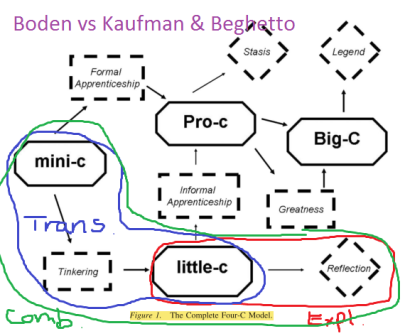
\includegraphics[width=\linewidth]{images/4CBoden.png}
\caption[Kaufman vs Boden]{Kaufman's 4 C Model vs. Boden}
\label{fig:4CB}
\end{figure}

\todo{comparison table Poincare, Wallas, Polya, CC?}

We had previously differentiated between creative computing and computational creativity:

\begin{quote}
Intuitively the former is about doing computations in a creative way, while the latter is about achieving creativity through computation. You can think of the latter falling into the artificial intelligence category (using formal computational methods to mimic creativity as a human trait, see also [18]) and the former being a more poetic endeavour of how the computing itself is done, no matter what the actual purpose of the program is. \autocite{Hugill2013}
\end{quote}

The differences are subtle but clear.

\begin{table}[htbp]
\centering
\begin{tabular}{|l|p{5cm}|l|}
\hline
\textbf{Creative Computing} & \textbf{Digital Humanities} & \textbf{Computational Creativity} \\ \hline
Motivation  & Design & Intentionality \\ \hline
Ideation & Curation, Analysis, Editing, Modeling and Networks, Infrastructure & Framing \\ \hline
Implementation & Computation, Processing & Process \\ \hline
Operation & Versioning, Prototyping, Failures & Product \\ \hline
\end{tabular}
\caption[Creative Computing vs Digital Humanities vs Computational Creativity]{Comparison of Creative Computing vs Digital Humanities vs Computational Creativity}
\end{table}

\begin{table}[htbp]
\centering
\begin{tabular}{|l|l|l|}
\hline
\textbf{4 step model} & \textbf{4 P Model} & \textbf{Problem Solving} \\ \hline
Preparation   & Person         & Understand  \\ \hline
Incubation    & Press/Context  & Plan        \\ \hline
Illumination  & Process        & Carry Out   \\ \hline
Verification  & Product        & Look back   \\ \hline
\end{tabular}
\caption[4 Step Model vs 4 P Model vs Problem Solving]{Comparison of 4 Step Model vs 4 P Model vs Problem Solving}
\end{table}

\begin{fcom}
How does ethics fit into this?
\end{fcom}





\section{Pataphysics}


\subsection{and Creativity}

The creative process normally involves a move from the known to the unknown and sometimes from the named to the unnamed. In bringing something new into existence, the human qualities of openness and tolerance of ambiguity are generally regarded as highly desirable. We may define creativity as \textbf{the ability to use original ideas to create something new and surprising of value}. We generally speak of creative `ideas' rather than `products', which merely provide evidence of a creative process that has already taken place. Both the originality and the value of an idea are evaluated using subjective criteria. \textbf{Pataphysics}, which represents an extreme form of subjectivity, is therefore a highly appropriate framework within which to encourage and enable creative thinking and operations.

Both the originality and the value of a creative idea are always evaluated using purely subjective criteria. Pataphysics, which represents an extreme form of subjectivity, is therefore a highly appropriate framework within which to encourage and enable creative thinking and operations.

\begin{quote}
  The ambiguity of experience is the hallmark of creativity, that is captured in the essence of pataphysics. Traversing the representations of this ambiguity using algorithms inspired by the syzygy, clinamen and anomaly of pataphysics, using a panalogical mechanism applied to metadata, should be able to humanize and even poeticize the experience of searching the Web. \autocite{Hendler2013}
\end{quote}

Pataphysics is highly subjective and particular and is as such very suitable for this kind of transformation from relevant to creative.

\begin{quote}
  [Pataphysics] can only be defined in a new undiscovered language because too obvious: tautology. \autocite{Baudrillard2007}
\end{quote}

It is instructive to overlay these ideas on existing theories of creativity. Margaret Boden \autocite{Boden2003}\marginpar{see section baalh}, for example, has defined \textbf{P-creativity} (short for psychological creativity) as the personal kind of creativity that is novel in respect to the individual mind and \textbf{H-creativity} (short for historical creativity) as fundamentally novel in respect to the whole of human history. This allows for subjective evaluation of any idea.

Using Boden's definition we can call an idea `new' if it is new to the individual who came up with it, making the idea P-creative. We can say that a creative idea can be seen from two perspectives: the subjective (P-creative) and the objective (H-creative) view. She argues that constraints support creativity, and are even essential for it to happen. ``Constraints map out a territory of structural possibilities which can then be explored, and perhaps transformed to give another one'' \autocite[p.82]{Boden2003}.

This echoes the ideas of groups such as the \textbf{Oulipo} (which began as a Sub-Commission of the Collège de $'$Pataphysique), who investigate `potential literature' by creating constraints that frequently have a ludic element. Various other groups, the Ou-x-Pos, perform similar operations in fields as diverse as cinema, politics, music and cooking \autocite{Motte2007}.

Boden's conceptual space is the ``territory of structural possibilities''. So, the conceptual space of a teacup might be that it is meant to carry a certain amount of tea without breaking or burning fingers. It wouldn't be wise to create a teacup made out of paper. But whether we make a cup out of glass or porcelain, or how we shape the cup or the handle is pretty much up the individual's creativity. Being able to move around in this conceptual space, experiment (in thought or in reality) and play with different ideas while still following a given set of constraints is a good starting point for creativity to happen. Boden defines three sub-types of creativity.

The Oulipo similarly classifies its conceptual space under two broad headings: the synthetic and the analytic:

\begin{quote}
  […] In the research which the Oulipo proposes to undertake, one may distinguish two principal tendencies, oriented respectively towards Analysis and Synthesis. The analytic tendency investigates works from the past in order to find possibilities that often exceed those their authors had anticipated. […] The synthetic tendency is more ambitious: it constitutes the essential vocation of the Oulipo. It's a question of developing new possibilities unknown to our predecessors. This is the case, for example, of [Raymond Queneau's] 100,000,000,000,000 Poems or the Boolean haikus. \autocite[p.27]{Motte2007}
\end{quote}

Later writings develop these ideas in more detail. La Littérature Potentielle \textbf{Oulipo1973}, is divided into several sections, dealing with clusters of methods, that include: anoulipisms (analytical oulipisms, such as combinatorial literature); use of preexisting structures such as lipograms (omitting a letter or letters), palindromes and snowballs (in which each successive word adds or subtracts a letter), homophonic translation, tautogram, and definitional literature; lexical, syntactic, or prosodic manipulations (such as the celebrated S+7, in which each substantive is replaced by the seventh word after it in a standard dictionary); lexicographical or prosodic synthoulipisms (early algorithmic methods); and perimathematical synthoulipisms (such as the Boolean poetry and combinatorial works already mentioned).

Boden links her three aspects of creativity to three sorts of surprise. She says that creative ideas are surprising because they go against our expectations. ``The more expectations are disappointed, the more difficult it is to see the link between old and new.'' \autocite[p.84]{Boden2003} This suggests that fewer \textbf{expectations} (an open mind) allow creativity to happen more easily. Empirical experiences form expectations, which hinder our ability to accept creative ideas when they happen. In order to be able to recognise creative ideas we need to be able to see what they all have in common and in what way they differ and not reject unusual, unexpected ones.

\begin{quote}
  ``Unless someone realizes the structure which old and new spaces have in common, the new idea cannot be seen as the solution to the old problem. Without some appreciation of shared constraints, it cannot even be seen as the solution to a new problem intelligibly connected with the previous one.'' \autocite[p.84]{Boden2003}
\end{quote}

It is clear that the Oulipo has a similar approach in its theorising of potential literature. Releasing creativity through constraint is its essential raison d'être.

This is not to say that experience and knowledge are necessarily bad for creativity. To appreciate creativity we need to be knowledgeable in the relevant domain to be able to recognise old and new connections and transformations. But we also need a certain level of openness and tolerance for ambiguity to overcome our expectations. Perhaps it is for this reason that `creative people' are often assumed to have particular personality traits. Sternberg \autocite{Sternberg1999, Sternberg1999}, for example, proposes that these comprise: independence of judgement, self-confidence, and attraction to complexity, aesthetic orientation, and tolerance for ambiguity, openness to experience, psychoticism, risk taking, androgyny, perfectionism, persistence, resilience, and self-efficacy. More empirically, Heilman, Nadeau and Beversdorf \autocite{Heilman2003} have investigated the possible brain mechanisms involved in creative innovation. While a certain level of domain specific knowledge and special skills are necessary components of creativity, they point out that ``co-activation and communication between regions of the brain that ordinarily are not strongly connected'' might be equally important.

Newell, Shaw and Simon add to the above with their report on the creative thinking process \autocite{Newell1963}. They identify three main conditions for creativity: the use of imagery in problem solving; the relation of unconventionality to creativity; and the role of hindsight in the discovery of new heuristics. Other issues they point out are abstraction and generalisation. So, for example, poets transform the grammar of their conceptual space (in this case, language) to create new sentence structures in a poetic form. By doing so, they go against the expectations, the possibilities of the language and cause surprise. Some people might not understand the transformations and therefore the jokes or beauty of a poem simply because they are either not able to recognise connections between the old and newly transformed elements (maybe due to a lack of knowledge in the poems topic or in that particular language) or because they do not want to accept unconventional methods.

Consider the following table, which compares some of the key ideas of creativity \autocite{Boden2003, Indurkhya, Koestler1964} with the main pataphysical operations. It will be seen that pataphysics succeeds in bringing into sharp relief the more generalised scientific ideas. The pataphysical terms are taken from the natural sciences or philosophy, but always with an ironic twist, betraying their underlying humour. They connect quite strongly with the primary descriptors of creativity, while adding a certain layer of jouissance. \textbf{Pataphysics is self-avowedly useless, but its principles may prove surprisingly useful within this context.}

\begin{table}[htb]
  \begin{tabu}{XX}
  \toprule
  \textbf{CREATIVITY}
  &
  \textbf{PATAPHYSICS}
  \\ \midrule
  \textbf{Combinational}: Juxtaposition of dissimilar, bisociation, deconceptualisation
  &
  \textbf{Antinomy}: Symmetry, duality, mutually incompatible, contradicting, simultaneous existence of mutually exclusive opposites
  \par
  \textbf{Syzygy}: Alignment of three celestial bodies in a
  straight line, pun, conjunction of things, something unexpected
  and surprising
  \\ \midrule
  \textbf{Exploratory}: Noticing new things in old places
  &
  \textbf{Anomaly}: Exceptions, equality
  \\ \midrule
  \textbf{Transformative}: Making new thoughts possible by transforming old conceptual space, altering its own rules
  &
  \textbf{Clinamen}: Unpredictable swerve, the smallest possible aberration that can make the greatest possible difference
  \\
  \bottomrule
  \end{tabu}
\caption[Creativity vs Pataphysics]{Creativity vs Pataphysics}
\label{tab:creatpata}
\end{table}


\subsection{and Computers}

\begin{draft}
  ANDREW:\\
  Since our solutions will be imaginary, our aim is not so much to have the computer generate creative artefacts as to engage in a creative dialogue with the user. Therefore, we do not intend to move as close to artificial intelligence as Colton's framework seems to suggest. In the pataphysical universe, ideas such as `human skill', `human imagination' and `human appreciation' are too generalised to be useful. One may very well ask: which human? And when, where and even why? Rather, our project will aim to produce an exceptional computational entity that consistently generates surprising and novel provocations to the users, who in turn may navigate and modify these by deploying their own skills, appreciation and imagination. The relationship between the two will develop quite rapidly into one of mutual subversion since, however apparent the `rules of the game' may become, the outcomes will always be particular or exceptional.
\end{draft}

We are not the first people to attempt to apply pataphysical ideas in computer science. Johanna Drucker focused specifically on the cleft between formal logic and subjective judgement. She introduced the discipline of `Speculative Computing' as a solution to that problem \autocite{Drucker2007}. The concept can be understood as a criticism of mechanistic, logical approaches that distinguish between subject and object.

\begin{quote}
  Speculative computing takes seriously the destabilization of all categories of entity, identity, object, subject, interactivity, process, or instrument. In short, it rejects mechanistic, instrumental, and formally logical approaches, replacing them with concepts of autopoiesis (contingent interdependency), quantum poetics and emergent systems, heteroglossia, indeterminacy and potentiality, intersubjectivity, and deformance. Digital Humanities is focused on texts, images, meanings, and means. Speculative Computing engages with interpretation and aesthetic provocation. \autocite[p.29]{Drucker2009}
\end{quote}

For Drucker, aesthesis (ambiguous and subjective knowledge) is fundamentally opposed to mathesis (formal objective logic) and subjectivity is always in opposition to objectivity. Knowledge is a matter of interpretation of information, which can be represented digitally as data and metadata. She introduces what she calls a \textbf{'patacritical'} method of including exceptions as rules, even if repeatability and reliability are compromised. Bugs and glitches are privileged over functionality, and are ``valuable to speculation in a substantive, not trivial, sense.'' As she says: ``$'$Pataphysics inverts the scientific method, proceeding from and sustaining exceptions and unique cases'' \autocite{Drucker2007}.

In order to break out of the formal logic and defined parameters of computer science, she asserts, we need speculative capabilities and pataphysics. ``The goal of pataphysical and speculative computing is to keep digital humanities from falling into mere technical application of standard practices.'' She links interface design with other speculative computing principles, and refers to Kant's idea of art as \textbf{'purposiveness without purpose'}. She says that the appreciation of design as a thing in itself (regardless of utility) is a goal of speculative aesthetics.

The projects Johanna Drucker describes in her book SpecLab \autocite{Drucker2009}  could certainly be considered related work. Not only in their theoretical foundations but also in some aspects of their implementation. One project in particular is worth mentioning here: the $'$Patacritical Demon, an ``interactive tool for exposing the structures that underlie our interpretations of text'', although it remained a purely conceptual piece of work and was never implemented. Her idea if the ``patacritical'' method is quite interesting. Pataphysical exceptions and anomalies can thus be justified in a computational system. But it is not just this concept that deserves mention here.
Her ideas on structured data, metadata and knowledge representation link very nicely into my project. How can we represent and structure data so that it does not lose its subjectivity, context and meaning? Her reference to graphical analogies is inspiring in that regard as well. I am certain I will refer back to her concepts throughout my thesis.


\section{Patalgorithms}

The proposed concept for a pataphysical algorithm requires precise data structures to represent the transformations that have taken place during the pataphysicalisation, such as the patadata. The system’s index has to be adapted to accommodate this new type of data structure. It also needs to be flexible enough to allow algorithms to fit in at different stages or locations of the system, for example the inverted-index, ranking functions or query itself.
Whilst this new style of algorithm has been proposed, current architectures are not capable of supporting them. As such a new flexible component-based software architecture has been proposed which will allow for a range of different style systems to be developed with little overhead. As such improving the chance of creative outcomes occurring in a different way.

\begin{draft}
  Linking back to some of the creative, pataphysical concepts we have discussed earlier, let us put some of the ideas for our tool into perspective. The constraints for our conceptual space are the pataphysical rules that we want to apply to our data. We use those rules to explore, combine and transform our space; giving us the flexibility and freedom we need to find interesting results.

  We developed the idea of pataphysicalising data as the process of applying such pataphysical rules in order to produce creative search results. This pataphysicalisation process forms a central component of our system (see Figure~\ref{fig:patasearch01}) and influences all areas of the search tool.

  \todo{redraw figure}

  \begin{figure}[htb] % (here, top, bottom, page)
    \centering
    
\includegraphics[width=\linewidth]{images/patasearch01}
  \caption[Pata central]{Pata central}
  \label{fig:patasearch01}
  \end{figure}

  \begin{figure}[htb] % (here, top, bottom, page)
    \centering
    % \def\svgwidth{\columnwidth}
    \input{images/patasearch01.pdf_tex}
  \caption[Pata central]{Pata central}
  \label{fig:patasearch02}
  \end{figure}
\end{draft}

\subsection{Pataphylicalisation}

The conceptual space for our project is `pataphysical Web searching'. There are some very simple rules or constraints that form an initial definition of the project. For example it is clear that we want to search the World Wide Web (rather than a library database), that we want to return a list of search results (and not a pile of books) and that we want the search process and its results to be creative/pataphysical (rather than relevant).  In a more technical sense, we have the query term (s), the index (of all web pages that we have crawled) and some pataphysical rules in our conceptual space. How we structure our search system, how we format the index or how we go about finding our results, is not in our conceptual space however. We can explore the space to its limits and we can transform it if we want to or feel like we need to. Our pataphysical rule set will include methods for transforming the space. By applying pataphysical rules to find results to our query we are pataphysicalising the query.

Definitions:
\begin{description}
  \item [To pataphysicalise] (verb) – applying pataphysical transformations
  \item [Pataphysicalisation] (noun) – the process of pataphysicalising
  \item [Patadata] (noun) – any data which has been pataphysicalised
\end{description}

But what exactly does the process of pataphysicalisation include? The kinds of transformations we are thinking of could be for example replacing or adding to the query term (s) with synonyms, antonyms, opposites, syzygies, clinamens etc. This can be done with the help of thesauri or dictionaries and ontologies. Whether we pataphysicalise our query term (s), the index or the results does not matter at this point. They are all possible and will maybe be done all at the same time (see figure~\ref{fig:patasearch02} below). We can consider the possibility of a `patametric index', rather than a parametric index or a `patasaurus' (pataphysical thesaurus/ontology).

\begin{figure}[htb] % (here, top, bottom, page)
  \centering
  \def\svgwidth{\columnwidth}
  \input{images/pataphysicalisation.pdf_tex}
\caption[Pataphysicalisation]{Pataphysicalisation}
\label{fig:patasearch02f}
\end{figure}

\begin{quote}
  Arguably, few other textual forms will have greater impact on the way we read, receive, search, access, use and engage with the primary materials of humanities studies than the metadata structures that organize and present that knowledge in digital form. \autocite[p.9]{Drucker2009}
\end{quote}


\subsection{Patadata}

The idea of patadata is derived from the idea below:\\
Physics $\to$ Metaphysics $\to$ Pataphysics\\
Data $\to$ Metadata $\to$ Patadata

Patadata will allow us to engage with digital knowledge in a more creative way even. If metadata helps us organise information semantically then patadata is for organising information pataphysically. If metadata is objective then patadata is subjective. Drucker also points out that ``many information structures have graphical analogies and can be understood as diagrams that organise the relations of elements within the whole.'' \autocite[p.16]{Drucker2009} So maybe patadata could allow us to represent these graphical analogies in some way? An alphabetical list is a typical model for representing text data sets for example. Or an otherwise ranked list, a tree structure, a matrix, a one-to-many relationship, etc. But is a ranked list really the best way to represent search results? Ranking itself seems unpataphysical. It contradicts the philosophy of pataphysics, although we can argue that this contradiction makes it pataphysical again. Maybe this dilemma can be solved simply by adopting another type of graphical analogy to structure the results such as a tree structure instead of a ranked list.

Example: Let's say our patadata is represented by a list of keywords that each stands for a pataphysicalisation of the original query term. This list is added to each item in the index.

Query      = `Tree'\\
Patadata = [Tree (equivalent),  Car (opposite), Paper (antinomy),\\ Narwhal (anomaly), Book (syzygy), Venus Fly Trap (clinamen)]

Query      = `Sun God Ra'\\
Patadata = [Sun God Ra (equivalent), Slave (opposite), Holiday (antinomy),\\ Blue Balloon (anomaly), Pyramid (syzygy), Sphinx (clinamen)]


\subsection{Ranking --- Pranking?}

In traditional Web search, ranking signals contribute to the improvement of the ranking process. These can be content signals or structural signals. Content signals are referring to anything that is concerned with the text and content of a page. This could be simple word counts or the format of text such as headings and font weights. The structural signals are more concerned about the linked structure of pages. They look at incoming and outgoing links on pages. There are also Web usage signals that can contribute to ranking algorithms such as the clickstream. This also includes ideas such as the Facebook `like' button or the Google `+1' button which could be seen as direct user relevance feedback.

Ranking can be done at different stages of the search process. Depending on how the index is formatted and what information can be pre-computed at that stage, the ranking algorithm evaluates every Web page for relevance and returns them in order. There exist lots of different approaches on ranking, including PageRank \autocite{Brin1998} and HITS \autocite{Kleinberg1999}, which both analyse the link structure of the World Wide Web. They analyse the incoming and outgoing links on pages. PageRank for example assigns a numerical weight to each document, where each link counts as a vote of support in a sense. It is executed at indexing time, so the ranks are stored with each page directly in the index. HITS stands for `Hyperlink Induced Topic Search' and its basic features are the use of so called hubs and authority pages. It is executed at query time. Pages that have many incoming links are called authorities and pages with many outgoing links are called hubs.

Given a query term X, what is considered a relevant match though? Do we simply return a list of Web pages where X appears in the heading of each page? It is obviously not that easy. Several ranking signals are combined together; Google states that they use over 200 signals including PageRank and they personalise results using signals such as the web history and location (Google n.d.).
What kinds of ranking signals do we need for our pataphysical Web search tool? We could say that a page Y is relevant if it matches the patadata for query X. So, for example, Y would be a relevant result if it is a clinamen or syzygy to X. The more patadata matches there are the higher the ranking maybe. We don't necessarily have to assign a numerical ranking value to each page. Depending on how we structure our results page that might not be necessary. Shuffling the results list or the results tree could be an option.

\begin{draft}
  \section{User experience}

  Whilst developing a system that returns creative results to the end user has numerous advantages, the assumptions that are made about and the decisions we take for the user must still be considered. For example, presume that the user inputs a search request `The Cat in the Hat' after reading a Dr.\ Seuss book to their child, and the system employs an anomalous method on the query and searched `sunglasses'. Whilst there is logic to the new search request, it is anomalous to the initial request, if the user receives these results without being told what method was used, the results will appear random, and therefore are likely to be detrimental to the user. Therefore the level of interaction the user has with the system and the feedback the system gives to the user on decisions it is making will have a large influence on the overall effectiveness and appreciation of the search tool. A quick and simple solution to this problem would be to add an icon to the side of each search result which displays how the original query was pataphysicalised.

  \begin{figure}[htb] % (here, top, bottom, page)
    \centering
    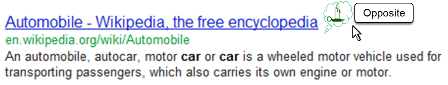
\includegraphics[width=\linewidth]{images/resultexample}
  \caption[Feedback button]{Feedback button}
  \label{fig:feedback}
  \end{figure}

  The above image (figure~\ref{fig:feedback}) shows an example of how this could be implemented. The little green candle (a reference to pataphysics in itself by the way) shows a pop-up note when hovered over with the mouse pointer. In this case the original query could have been `tree' and `car' was returned as an opposite to that.
\end{draft}



% -----------------------------------------
% \begin{fcom}
% \section{Information retrieval systems}
%
% Information retrieval is one of the common processes that a person carries out day-to-day, usually without even thinking about. The amount of information that a human comes in contact with on a daily basis is overwhelming and as such we have developed very sophisticated methods of finding the \textbf{relevant information} instantaneously. However, it is also possible to see how this relates to a large number of commonly used computer systems.
%
% "Information retrieval (IR) is finding material (usually documents) of an unstructured nature (usually text) that satisfies an information need from within large collections (usually on local computer servers or on the Internet)." \autocite{Nickerson1999}
%
% It is important to note, that whilst a large proportion of IR is focused on \textbf{Web search engines}, this is not the only application. The reason that such a large focus is on this area, is due to the unique challenges it holds, huge quantities of \textbf{unstructured data} which changes over time and can be in a number of formats. The true aim of any research into search engines is that it can be applied back to the general field of IR and enhance a much larger ecosystem of systems.
%
% However, research in all of IR focuses on arbitrary values of success, called \textbf{precision and recall}, the fraction of retrieved instances that are relevant and the fraction of relevant instances that are retrieved respectively. Whilst these measures are logical, they are arbitrary due to the \textbf{subjectiveness of relevance}. And due to the clinical nature of the measures, returning results that are partially related to the request would be detrimental to the perceived quality of the system, irrelevant of the insightful knowledge it may provide.
%
% It is possible, under this definition, that there is no ranking function; such is the case for the Boolean model. Whilst this may not appear logical when considering search engines, there are a number of cases where returning all possible results which match our `need' without bias can be useful. It is not however, possible for an IR system to exist without any of the other components.
%
% \subsection{Beyond the realm of traditional IR systems}
%
% Most modern Web search engines, excluding semantic search engines, have a similar architecture, irrelevant of the IR model they are based on (see figure 1). The main reason for this is due to the \textbf{generic data-store} at the heart of them, the \textbf{inverted-index}, which is a very efficient method of storing and searching over the contents of documents.
%
% \todo{redo archticeture diagram}
% \begin{figure}[htb] % (here, top, bottom, page)
% \centering
% 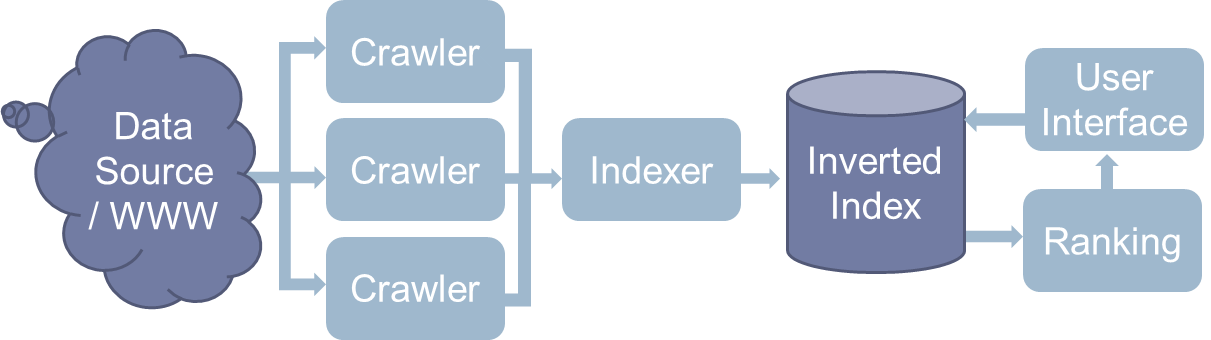
\includegraphics[width=\linewidth]{images/patasearch03}
% \caption[Traditional IR system]{Traditional IR system}
% \label{fig:patasearch03f}
% \end{figure}
%
% In an inverted index, the contents of a document are broken into various different combinations or terms by the indexer, and a link to the original document is stored with each of these terms. This means that when searching for a \textbf{keyword}, instead of having to look at every document and its contents, the system just looks for all terms that match the request and returns the various links that match. The inverted index is quick at retrieval; however, building the index is slower.
%
% Even with these characteristics, the inverted-index is not suitable with respect to any of the above definitions of creativity. We are only able to search over the contents of the document as they are, with \textbf{no understanding of their meaning}. As such, being able to implement pataphysical themes like clinamen or syzygy would be very challenging.
%
% It is possible to apply these concepts to a traditional search engine architecture, by modifying the user's search request. Hendler and Hugill \autocite{Hendler2011} suggest that by using 'panalogies' we can model patadata and as such apply pataphysical constructs to requests. In the proposal that is outlined, the system would be applied to work on the open Web, using results from commercial search engines, as well as domain specific systems such as the British Library.
%
% However, there is a limitation to such as system.  Whilst we can modify the initial request to something with a more creative twist, the system cannot make decisions based on the underlying content of the results. As such the quality of the results is limited by the quality of the indexer and not the search algorithm. Whilst this could be argued to be true in any search architecture, the index is built up of data that we wish to access directly, i.e. searching over the content to find a document that matches based on certain rules. With respect to creative search, it makes more sense that we look at how different parts of the document relate to each other, and other documents based upon underlying meaning and not pure text. Even with this in mind, such a system would be adventurous from a creative stand-point over current search engines, and would provide an interesting insight into how people would respond to such a system and how important the user interface would be in such a system.
%
% \subsubsection{Semantic search engines}
%
% \textbf{Semantic search engines} would therefore seem to be a more logical fit to a pataphysics inspired creative search engine as it will allow the creation of links between different documents based on more than the exact words used.
% The key difference between the architectures of traditional IR systems is the way that the data is stored and hence the indexing process. The majority of different semantic search systems use \textbf{RDF triples} as a way of storing data, based on Semantic Web ontologies.  In RDF, each entry to the data-store has the following attributes <<object>> <<relation>> <<value>>  - such as a blue balloon would be  <<balloon>> <<hasColour>> <<blue>>, this is not meant to represent the syntax of RDF; however, for this example, the relation of hasColour and the concept of blue being a colour would have to already have been defined.  However, trying to represent the concept of "12 blue balloons" requires even more relations and concepts to be defined; therefore, if we end up with a large amount of loosely related data, the number of concepts and relations defined will explode. However, if the data is tightly related, the amount of relations and concepts is much smaller and therefore easier to reason about.
%
% With the data stored in this format, \textbf{inference logic} and/or \textbf{fuzzy set theory} can be used to carry out searches over the data-set to return concepts that relate. These inference searches are slow and tend not to relate directly to documents, instead return a list of different concepts which can then be linked back to the documents. This is usually done with an inverted-index using traditional methods to return documents that match numerous combinations of the concepts.
%
% With this method, the trickiest part of the system is \textbf{indexing}, as a document must be related back to concepts that exist within the system already. If they do not exist in the system already, the concept must be found in an \textbf{ontology} that has already been defined, which then leads to the problem of ontology merging, or creating them from scratch.
%
% Whilst this clearly allows more for the concepts that we have defined for results to be creative, there are a number of issues that arise. The fact that once a document has been added to the system, the concepts are set in stone. Whilst the RDF store will evolve over time and hence change the concept results that emerge, the document's classifications are set in stone. This is not just a problem for a creative search engine, but for all semantic search engines as well.
%
% Also, within an ontology, different concepts tend to be linked with relations that are descriptive, such as <<isAn>>, <<hasColour>>, <<produces>> etc. However, these types of relations are not analogous with the pataphysical concepts that have been defined, and as such it is not immediately apparent how one could implement a syzygistic transformation of a search request using an RDF data store.
%
% As can be seen by looking at the two main search architectures, a new IR system architecture is needed; however, instead of defining it from the top down, the algorithms need to be defined first to allow maximum flexibility in the system to allow the definition of creativity to evolve over time.
%
% It is clear that any of these new algorithms, or ones that follow, will not be suitable for existing system architectures in IR research, and as such a new one will need to be defined. The question becomes, whether or not the architecture itself can help enhance the chance of providing creative search results. If so, would it be possible to abstract this so that it can be used in other types of systems to help allow creative computing to flourish in areas where it may not have been possible before. This is a tall order, and one that is not likely to come soon; however, developing an architecture that is as generic as possible can only aid this task.
%
% The concept of pataphysicalisation, using pataphysical methods to transform an object/idea, on the search request however, does appear to be an interesting place to start the search for a new architecture. Whilst argued above, it cannot be the end of the process due to the amount it constrains the possible creative outputs, the characteristics of such a system, how you would get users to interactive with such a system, as well as how they would respond to it, will give valuable insight into the areas that need to be addressed by both the algorithms and hence the architecture.
%
% A component based system architecture is therefore proposed to allow for greater flexibility in search engine development, whilst reducing the coupling between different parts of the system. This coupling tends to mean that for a new concept to be tried; large proportions of the entire search engine need to be re-developed. The use of standard interfaces, for different types of components, would therefore allow a generic harness to handle the communication between these different components and provide a seamless service to the end-user. The wiring of these components could be handled by a configuration file therefore allowing people to build systems without needing any explicit programming skills.
%
% Whilst this architecture itself does not explicitly improve the chance of creative results being returned, it will allow for new components to be tested in a full scale environment in an agile way and as such should allow for quicker testing. The harness is currently being developed, including a number of administration and monitoring tools inbuilt to aid analysis. The aim is to test the new architecture using a standard search engine and the Syzygy Surfer proposed by Hendler and Hugill\autocite{Hendler2011}.
%
% It is interesting to note how such a system could also be used in an educational environment to teach students how search engines work. Students could attempt to build systems using pre-built components and seeing how different arrangements of such components affect the outcome. This is very similar to the way that MIT has proposed to teach children how to program using the Scratch development environment2. More advanced students could also develop their own components to test out theories and improve their understanding of the base concepts of not just search engines, but the various fields that play a role in information retrieval systems.
%
% It is clear that this system could have great advantages outside of being a test-bed for new ideas, allowing for the easy development of search engines to suit the needs of all new types of problems, without the need for specific development of every component. Whilst this idea is still within its infancy, the potential is strong, and will be explored over time.
% \end{fcom}

\stopcontents[chapters]
